%%%%%%%%%%%%%%%%%%%%%%%%%%%%%%%%%%%%%%%%%
% Avi's Project Proposal
%
% Summer Research Project 
%
%%%%%%%%%%%%%%%%%%%%%%%%%%%%%%%%%%%%%%%%%

%----------------------------------------------------------------------------------------
%	PACKAGES AND DOCUMENT CONFIGURATIONS
%----------------------------------------------------------------------------------------

\documentclass{article}

\usepackage[version=3]{mhchem} % Package for chemical equation typesetting
\usepackage{siunitx} % Provides the \SI{}{} and \si{} command for typesetting SI units
\usepackage{graphicx} % Required for the inclusion of images
\usepackage{natbib} % Required to change bibliography style to APA
\usepackage{amsmath} % Required for some math elements 
\usepackage{gensymb}
\usepackage{ upgreek }


\setlength\parindent{0pt} % Removes all indentation from paragraphs

\renewcommand{\labelenumi}{\alph{enumi}.} % Make numbering in the enumerate environment by letter rather than number (e.g. section 6)

%\usepackage{times} % Uncomment to use the Times New Roman font


%Code packages
\usepackage{indentfirst}
\usepackage[utf8]{inputenc}
\usepackage{listings}
\usepackage{color}
% Code packages end


\usepackage[T1]{fontenc}
\usepackage[utf8]{inputenc}
\usepackage{authblk}


\makeatletter 
\newcommand\mynobreakpar{\par\nobreak\@afterheading} 
\makeatother


%----------------------------------------------------------------------------------------
%	DOCUMENT INFORMATION
%----------------------------------------------------------------------------------------

\title{Use of the Bayes Factor to Improve the Detection of Binary Black Hole Systems} % Title


%Jonah B. Kanner
\author[1]{Avi Vajpeyi }		 
\author[2]{Rory J. Smith \thanks{smith\textunderscore r@ligo.caltech.edu}} 
\author[2]{Jonah B. Kanner \thanks{jkanner@caltech.edu}}
\affil[1]{The College of Wooster, Wooster, OH 44691, USA}
\affil[2]{LIGO Laboratory, California Institute of Technology, Pasadena, CA 91125, USA}


\renewcommand\Authands{ and }

%\author{Avi \textsc{Vajpeyi}} % Author name

\date{\today} % Date for the report

\begin{document}

\maketitle % Insert the title, author and date


%have an understanding of what you will do and why the work is necessary or desirable
%It outlines the approach you will take to carry out your task
%It provides a schedule or time line for accomplishing the individual steps and overall goals of your project
%It encourages your mentor and his or her staff to make the arrangements necessary to accommodate you and your needs before your arrival




 \begin{abstract}
On September 14th, 2015, the Advanced LIGO detected the first gravitational wave \cite{DetectionPaper}. The detected wave had a very large Signal to Noise Ratio value, which made it stand out from the rest of the candidate events. This paper investigates an alternative detection statistic, involving the `Bayes Factor.' This detection statistic might prove to be more robust than SNR, as it may be able better to discern between strains due to gravitational waves, and strains due to noise. This study of the new detection statistic is focused on binary black hole systems. 


\end{abstract}  




%----------------------------------------------------------------------------------------
%	SECTION 1
%----------------------------------------------------------------------------------------

\section{Introduction}

\indent The completion of the two Advanced Laser Interferometer Gravitational-Wave Observatories (aLIGO) has led to the discovery of a gravitational-wave signal \cite{DetectionPaper}. This paper deals with a new detection statistic, involving Bayesian statistics, to rank the different candidate events (the strains in the data sets that could be due to gravitational waves). The candidate events we focus on are from binary black hole systems as they are believed to be common in the Universe \cite{NumDetections}.\\

 Before we study this new detection statistic, we will discuss how data is currently being recorded and analysed.\\


\subsection{Introduction to the physics of LIGO} \label{section:intro}


 
 % How Ligo detects signals
 \indent Each of the aLIGO observatories uses a modified Michaelson Interferometer that measures the difference in the length of the orthogonal arms of the observatory to detect the presence of a gravitational wave \cite{DetectionPaper}. On passing, a gravitational wave induces a difference in the length of the arms which is measured as a phase shift in the circulating laser light.\\
 
  % how signal is found in data
  \indent To determine if data recorded by LIGO store gravitational wave information, the data is processed with two search techniques. One search looks for generic transient waveforms ( unmodelled or unexpected waveforms) in data \cite{Enia}. The second is a match filtered search that compares the data with templates of waveforms generated by general relativity \cite{Enia}.\\
  
  % Discussion on how background noise is removed with time shifts, and how data is ranked 
  
  %The background noise can result with strains in the data similar to strains from gravitational waves \cite{DetectionPaper}.
  
  \indent Both the search processes are made challenging due to the background noise present in the data.  This background noise can result from defects in a mirror, the uncertainty in the number of photons travelling in a the laser beam (shot noise), seismic activity, or even thermal noise generated by the Brownian motion of electrons inside circuits \cite{RSmith}. To separate  strains caused by background noise from those caused by gravitational waves, the data from one LIGO observatory is compared with another LIGO observatory's data \cite{DetectionPaper}. To compare the data sets, one of the them can be time-shifted so that it matches the data in the other detector over the light-travel time between the detectors. That is, one data set can be time-shifted so that both of the data sets lie along the same interval of time.\\
  
  %After making the necessary time shift, events present in one data set but not the other become apparent. If a strain is not present in both data sets, the strain may have resulted from noise in one of the detectors, as a gravitational wave strain would be observed in both detectors \cite{DetectionPaper}. Hence, all the strains that cannot be correlated with a data set taken from another observatory are discounted as strains due to noise \cite{DetectionPaper}. This process cuts a majority of the strains that may have been present due to noise\cite{DetectionPaper}. We attempt to discount any remaining noise-strains by implementing a detection statistic to rank the strains according to the likelihood that the strain resulted from a gravitational wave.\\
  
    After making the necessary time shift, events present in one data set but not the other become apparent. This process cuts a majority of the strains that may have been present due to noise \cite{DetectionPaper}. We attempt to discount any remaining noise-strains by implementing a detection statistic to rank the strains according to the likelihood that the strain resulted from a gravitational wave.\\
  
    % Talk about Time-frequency morphology classes, and how certain classes can be discounted? That is more specific to Generic...
  
  % SNR as a detection statistic 
  \indent The detection statistic currently being used to rank strains according to the maximum likelihood of it being due to a gravitational wave is the signal-to-noise ratio (SNR) detection technique \cite{Enia}. This method compares the power of the strain signal to the power of the remaining noise at a given point \cite{RSmith}. Although the power of the noise is difficult to calculate, we know that this ranking process can make some gravitational wave strains stand out, as seen from the Fig~\ref{Fig:Detection}.  However, we believe that this method lacks the sensitivity necessary to detect some gravitational waves that do not have SNR values as high as those of GW150914. Hence we would like to investigate an alternate detection statistic, specifically one that compares the relative probability that a data set contains a strain due to a gravitational wave to the probability that the data just contains noise. This ratio is known as the Bayes Factor.\\
  
  
  Additionally, the templates that are used in the matched filtered searches account for only a small subset of the vast possibility of gravitational wave signals. This might result with some gravitational waves signals that do not have templates to be left undetected.  In contrast, the LALInference program, which is what will be used to implement the new detection statistic, uses templates that can describe a far bigger set of signals. Hence, the Bayes factor might prove to be more sensitive than SNR, as we will have more information about the signal.
  %Additionally, it is believed that this detection statistic might help increase the detection rate of gravitational waves by a factor of 10, as  [Not sure what to cite here - could not find mention of this in Enia's paper]. 
  
  
  
\begin{figure}[h]
	\centering
	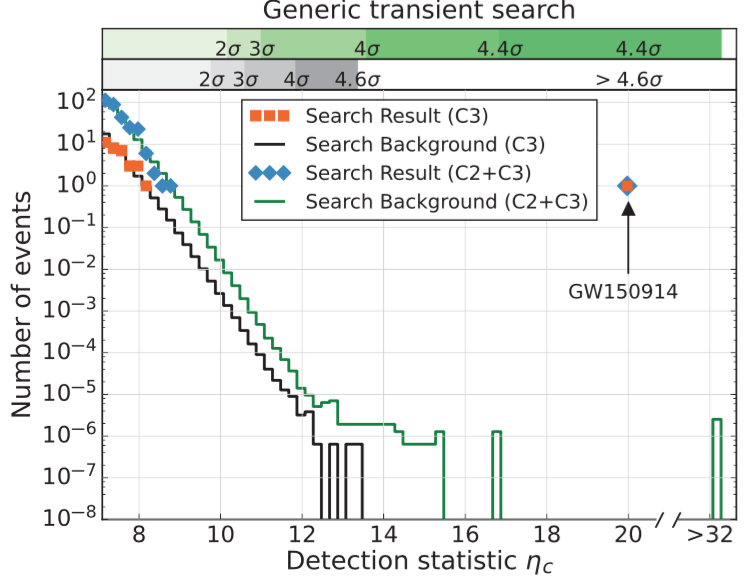
\includegraphics[width=0.5\textwidth]{Figures/DetectionInGenericTransientSearch}
	\caption{Search results of the generic transit search in which the first gravitational wave signal, marked GW150914, was detected. The wave strain of GW150914 stands out as the strongest strain in the entire search. SNR was used in this search to calculate the background noise and the events. Figure taken from \cite{DetectionPaper}}
	 \label{Fig:Detection}
\end{figure}

 
 
  %----------------------------------------------------------------------------------------
  %	Progress Report
  %----------------------------------------------------------------------------------------
  
  

 
 
 %----------------------------------------------------------------------------------------
 %	Objectives 
 %----------------------------------------------------------------------------------------
 
 \subsection{Introduction to Bayesian Inference for Gravitational Wave Analysis}
 \label{section:introToBayes}
 
To compute the Bayes factor between two hypotheses, we need to first define the models we are comparing. The models are descriptions of the data $d(t)$, which contains either only noise, or noise along with a gravitational wave signal, parametrized by a certain vector $\vec{\theta}$. The data $d(t)$ is recorded in the time domain, but can be written in the frequency domain at the frequency $f$ of the detector as $\tilde{d}(f)= \tilde{h}(f)+\tilde{n}(f).$ The Fourier Transformed data $\tilde{d}(f)$ is at times easier to work with. \\

\begin{figure}[h]
	\centering
	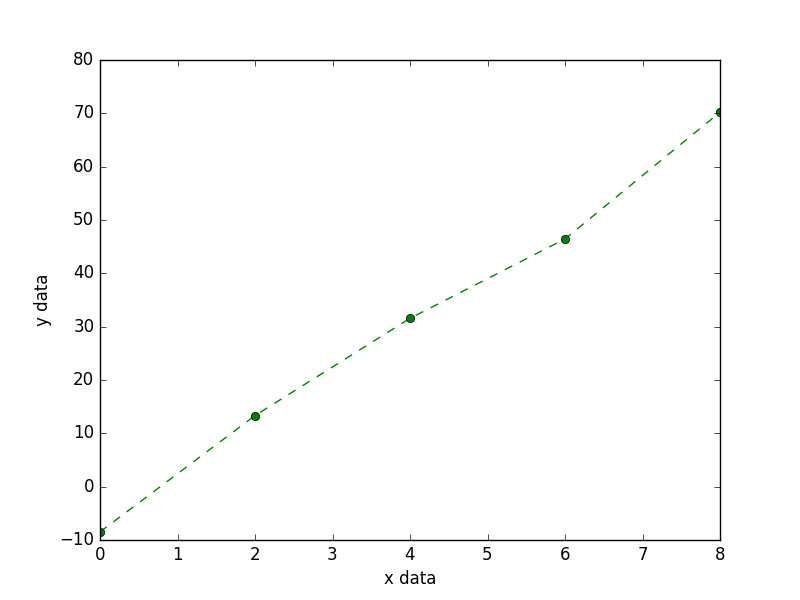
\includegraphics[width=0.5\textwidth]{Figures/rawData.png}
	\caption{Plot of the raw data that is used in this example question.}
	\label{Fig:Detection}
\end{figure}


The parameter vector $\vec{\theta}$ contains information on several quantities describing the binary black hole system such as the masses of the black holes ($m_1, m_2$), their spin vectors, and the distance of the black holes from Earth \cite{BaeStats}. This vector also contains quantities such as the GPS time at the geocentre at which the gravitational wave passes the Earth ($t_0$), and the phase of the signal at this time ($\phi_0)$ \cite{BaeStats}. The observed signal is actually dependant on fifteen quantities \cite{BaeStats}:
$$\vec{\theta} = \{ m_1, m_2, t_0, \phi_0, D_L, \alpha, \delta, \psi, \iota, \vec{s_1}, \vec{s_2} \}. $$
$\text{ }$\\
 The noise that is present in the data is assumed to be a Gaussian with a mean of zero, and a variance described by the noise spectral density of the data, $S_n (f)$, at a frequency $f$ \cite{BaeStats}. Under these standard assumptions, we can define the likelihood of noise to be given by the equation
  \begin{equation} \label{eq:noise}
 P(n(f)) \propto \frac{1}{\sqrt{2 \pi \sigma(f)^2} } \ e^{\frac{1}{2} \big(\frac{n(f)}{\sigma(f)}\big)^2},
  \end{equation}
  \noindent with $\mu = 0$ and $\sigma  = S_n (f)$.\\
 
 
 
 Finally, we can formally define the models we will use as:
\begin{itemize}
	\item $\mathcal{H}_{null}$: the noise model, which corresponds to the hypothesis that $d(t)$ contains only noise,
	$\mathcal{H}_{null}: d(t) = n(t)$.
	\item $\mathcal{H}_{GW}$: the gravitational wave signal model, which corresponds to the hypothesis that the data contains noise, and a gravitational wave signal parametrised by $\vec{\theta}$. Hence the model is defined by $\mathcal{H}_{GW}: d(t) = h(\vec{\theta},t) + n(t)$.
\end{itemize}
 
 
We can compare these two models by calculating the relative probabilities in the form of the posterior odds ratio $O_{GW, null}$ between the two of them, as explained in Ref~\cite{BaeStats}, 
  
  \begin{align} \label{eq:relProb}
  O_{GW, null} &= \frac{P(d|  \mathcal{H}_{GW})}{P(d|  \mathcal{H}_{null})} \  \frac{P(\mathcal{H}_{GW}) }{P(\mathcal{H}_{null})}  \nonumber\\
  &= B_{GW, null} \ \frac{P( \mathcal{H}_{GW}) }{P( \mathcal{H}_{null})},
  \end{align} 
  
   where $B_{GW, null}$ is the `Bayes' Factor,' which is equal to :\\
  \begin{equation} \label{eq:BayesFactorOrig}
  B_{GW, null} = \frac{P(d|  \mathcal{H}_{GW})}{P(d|  \mathcal{H}_{null})} \ .
  \end{equation}
 
It should be noted that the relative probability, Eq~\ref{eq:relProb}, and the Bayes factor, Eq~\ref{eq:BayesFactorOrig}, contain no reference to the signal parameters $\vec{\theta}$. Hence, the Bayes factor $B_{GW, null}$ can be calculated from our hypothesis, for any choice of model.\\

 To be able to account for the set of parameters $\vec{\theta}$ for a gravitational wave, the likelihood of the model $\mathcal{H}_{GW}$ needs to be marginalised over all the parameters, weighted by their prior probability distribution, giving the marginal likelihood or evidence, given by $P(d|\mathcal{H}_{GW})$  \cite{BaeStats}.\\
 

To calculate $P(d|\mathcal{H_{GW}})$, first we need to determine the \textit{posterior probability density function} (PDF). For gravitational wave analysis, the PDF of the parameters $\vec{\theta}$ is \cite{RSmith}:

%equation of PDF\\
\begin{equation} \label{eq:PDF}
p(\vec{\theta}|d, \mathcal{H}_{GW})  = \frac{p(\vec{\theta}| \mathcal{H}_{GW}) \ p(d|\vec{\theta},  \mathcal{H}_{GW})}  { p(d|\mathcal{H}_{GW})},
\end{equation} 

or in other terms, 

\begin{equation} \label{eq:englishTheorem}
{ Posterior \ Probability \ Density \ Function}  = \frac{ Prior  \times Likelihood}{Evidence}. \nonumber
\end{equation} 

In other words, in Eq~\ref{eq:PDF}, we have each model $ \mathcal{H}_{GW}$, to have a vector of parameters $\vec{\theta}$, with which we can calculate a `Prior' distribution of $P(\vec{\theta}| \mathcal{H}_{GW})$. This prior states what specific values the model $ \mathcal{H}_{GW}$ might be expected to take from the data set $d$. We also have $p(d|\vec{\theta},  \mathcal{H})$, which is the `likelihood' of the data, given that the model $ \mathcal{H}_{GW}$ is true. This likelihood can be calculated for a model $\mathcal{H}_{i}$ with
\begin{align}\label{eq:likelihood}
p(d|h, \mathcal{H}_{i}) & \propto \text{exp} \ \bigg[-\frac{1}{2} \ (d-h|d-h)\bigg] \nonumber \\ 
& \propto \text{exp} \ \bigg[-\frac{2}{T} \ \sum_{k>0} \frac{ | \tilde{d}(f_k) - \tilde{h}(f_k) | ^ 2 }{S(f_k)}\ \bigg],
\end{align}
as seen in Ref~\cite{BaeStats}. In this equation, the term $(d-h|d-h)$ is referred to as a noise-weighted inner product, which is a mathematical tool used often in signal analysis. The noise weighted inner product of two signals $A$ and $B$ can be calculated as shown in Ref~\cite{lindblom2008model}, $$(A|B) = 2 \int_{0}^{\infty} {\frac{\tilde{A}^* (f)  \tilde{B} (f)  +  \tilde{A} (f)  \tilde{B}^* (f) }{S_n(f)}}df. $$ Additionally, the term $T$ is the duration of the data that contains the signal of the gravitational wave. It is equal to the inverse of the size of the discrete frequency being stepped over: $df = 1/T$ \\





To finally solve for $p(d|\mathcal{H}_{GW})$, we rearrange Eq~\ref{eq:PDF} and integrate over $\vec{\theta}$, to get 

\begin{equation} \label{eq:evidence}
 p(d|\mathcal{H}_{GW})    = \int_{\Uptheta} p(\vec{\theta}| \mathcal{H}_{GW}) \ p(d|\vec{\theta},  \mathcal{H}_{GW}) d\vec{\theta},
\end{equation}


since the integral of the PDF, by definition of a probability density, is $$\int_{\Uptheta} p(\vec{\theta}|d, \mathcal{H}_{GW})\ d\vec{\theta}  = 1 .$$ \\

We can now use the value for $p(d|\mathcal{H}_{GW})$ from  Eq~\ref{eq:evidence}, and substitute it into our equation for the Bayes Factor, Eq~\ref{eq:BayesFactorOrig}. This Bayes' Factor may be able to better highlight the strains due to gravitational waves in our data.\\

We will demonstrate the use of the Bayes factor by generating a figure, like Fig~\ref{Fig:Detection}. However, instead of using SNR to calculate the background noise and rank the candidate events, the Bayes factor will be used. %This could raise the number of detections of gravitational waves generated by binary black hole systems. With more detections, we could have more data on the masses and spins of black holes in our Universe. With these results, we would be able to gain an estimate of the population of black holes in our Universe. [Not sure what to cite here - I got this from the project abstract]
 %----------------------------------------------------------------------------------------
 %	SECTION 3
 %----------------------------------------------------------------------------------------
 
 
 \section{Approach}
 The main objective of this project will be to assess the sensitivity of the Bayes' Factor to rank gravitational waves that might have been missed using SNR as the detection-statistic. This analysis will be done with a procedure that we will write, with the help of the LALInference program.\\
 
 We will begin by establishing the search background of the noise, with the help of the Bayes factor. This search background is made after time-shifting the data, as discussed in Section~\ref{section:intro}.  We will then inject gravitational wave signal into data sets, and use the new detection statistic to study if it can detect the waves. If the Bayes Factor is unable to detect the gravitational wave signal, we will study the thresholds at which the the gravitational wave signals can finally be detected with the Bayes factor. \\
 
 We will then study past data and see if the Bayes Factor detection statistic can help extract more gravitational waves signals from the noise in the various data sets. We will also study whether the new detection statistic will be able to detect gravitational waves from quieter events, that would appear as the background of SNR, as seen in Fig~\ref{Fig:Detection}.
 
 
 \section{Progress Report}
 
 In this section, results from the work from weeks 1-3 will be discussed.
 
 \subsection{A Simple Bayesian Statistics Calculation}
 
 Bayesian Statistics can get complicated to program. To understand programming techniques to compute the Bayes factor between two hypothesis and to evaluate the posterior densities for unknown parameters in models, we began the summer by studying a simple example. \\
 
 \begin{figure}[h]
 	\centering 	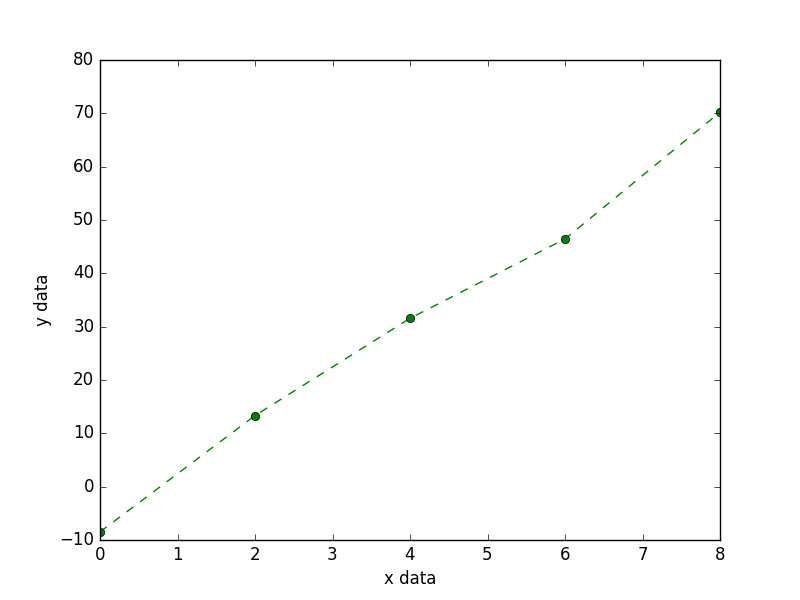
\includegraphics[width=0.7\textwidth]{Figures/rawData.png} 
 	\caption{Plots of the Posteriors}
 	\label{Fig:origData}
 \end{figure}
 
 
 In the example, there was some data $d(x)$ provided that had some Gaussian noise built in with a standard deviation of $\sigma = 5$. We were asked to fit the data with two models. The first model proposed that the data consists of a straight line passing through the origin and some noise, and the second model hypothesised that the data contains only noise. We this information, we can define the two models: \\
 \begin{itemize}
 	\item $\mathcal{H}_{m}$: the signal model, which corresponds to the hypothesis that $d(x)$ contains a line passing through the origin $(mx)$ and some Gaussian noise $n(x)$,
 	$$\mathcal{H}_{m}: d(x) = mx + n(x)$$.
 	\item $\mathcal{H}_{n}$: the noise model, which corresponds to the hypothesis that the data contains only Gaussian noise, and is defied as $$\mathcal{H}_{n}: d(x) = n(x)$$.
 \end{itemize}
 
 In both of the models, the noise can be defined by Gaussian as in the Eq~\ref{eq:noise}. In this case, we set $\sigma ^ 2 = 5$ and $\mu = 0$ to get: 
 \begin{equation}\label{eq:noiseMX}
 n(x) = \frac{1}{5 \sqrt{2 \pi} } \ e^{\frac{1}{2} (\frac{x}{5})^2}.
 \end{equation}
 
 

\begin{figure}[h]
	\centering
	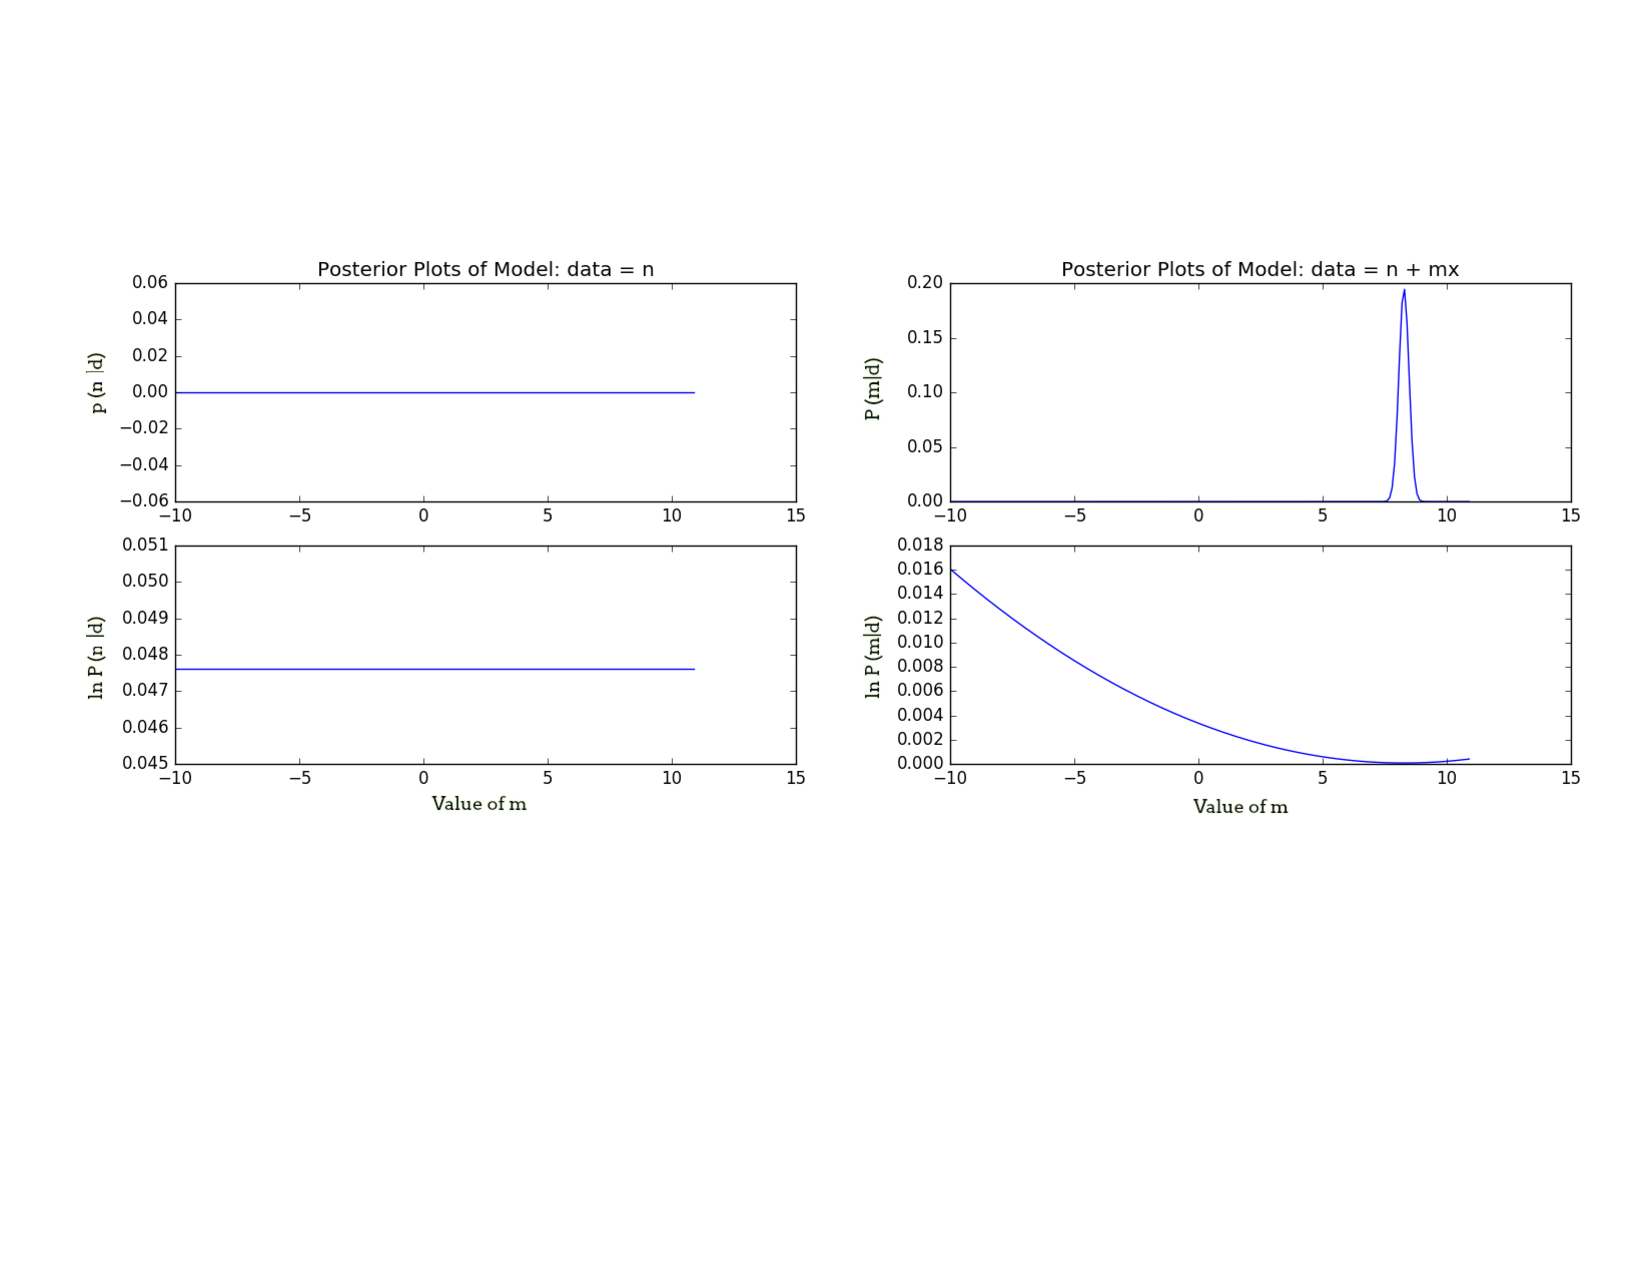
\includegraphics[width=1\textwidth]{Figures/exampleMXplot.pdf} 
	\caption{Plots of the Posteriors}
	\label{Fig:exampleMXplot}
\end{figure}
 
Modifying the equation for the calculation of the posterior density function, Equation~\ref{eq:PDF}, we calculated the PDF for $\mathcal{H}_{m}$ with 
\begin{equation} \label{eq:PDFforMX}
	P(m|d,\mathcal{H}_{m}:d(x) = mx + n(x))  = \frac{P(m| \mathcal{H}_{m}) \ P(d|m,  \mathcal{H}_{m})}  { P(d|\mathcal{H}_{m})} \ ,
\end{equation}
 and we calculated the posterior density for $\mathcal{H}_{n}$ with \begin{equation} \label{eq:PDFforMXnoise}
 P(m|d,\mathcal{H}_{n}:d(x) = n(x))  = \frac{P(m| \mathcal{H}_{n}) \ P(d|m,  \mathcal{H}_{n})}  { P(d|\mathcal{H}_{n})} \ .
 \end{equation} In both equations, we calculated the likelihood function using Eq~\ref{eq:likelihood}. For example, the likelihood for the noise model can be written as $$ P(d|d(x)=n(x)) \propto \text{exp} \ \bigg[ -\frac{1}{2} \sum_{i>0} \frac{| n(x_i)|^2}{\sigma}	\bigg]$$ 
 while the likelihood for the model $\mathcal{H}_{m}$ is  
 \begin{align*}
  P(d|d(x)=mx+n(x)) & = P(d|n(x)=d(x)-mx)\\
  &\propto \text{exp} \ \bigg[ -\frac{1}{2} \sum_{i>0} \frac{|d(x_i) - mx_i|^2}{\sigma}	\bigg]
 \end{align*}

  \noindent $\text{ }$\\
 
  Plots of the posterior densities for both the models can be seen in Figure~\ref{Fig:exampleMXplot}. Looking at the plot for the posterior distributions for the $\mathcal{H}_{m}$ model, we can see a peak at $7.6\pm 0.4$, which is what the most probable value for the slope of the line would be. Looking at the plots for the noise model, we see that the there is no regions of high probability, suggesting that the noise model does not fit the data well. \\
 

To see how well the the model $\mathcal{H}_{m}$ fits the data compared to model $\mathcal{H}_{n}$, we can compute the Bayes factors of the models. From Eq~\ref{eq:BayesFactorOrig}, we know that the Bayes factor is the ratio of the marginal likelihoods for the two models. Hence, in this case, the Bayes factor between the $\mathcal{H}_{m}$ and $\mathcal{H}_{n}$ models is $$B_{m,n} = \frac{P(d|\mathcal{H}_{m})}{P(d|\mathcal{H}_{n})} = \text{exp}\ [233170].$$ This value is very high, and hence, this tells us that the model $\mathcal{H}_{m}$ is a much more likely model than $\mathcal{H}_{n}$. Hence, from this, we can conclude that the given data $d(x)$ contains a line that masses through the origin and has a slope of $7.6\pm 0.4$ with some noise. In the next section, we will discuss how we can use Bayesian Inference to study gravitational wave strain data.\\


 \subsection{An Example of Bayesian Inference for Binary In-Spirals}
 
 As seen in the previous example, Bayesian inference can provide efficient and powerful approaches to model selection and parameter estimation. In this section, we describe the computational processes and theory needed to analyse some aLIGO strain data. We discuss how Bayesian inference can be used to calculate both the Bayes factor of the signal and the parameters that generated the signal. Note that this example uses gravitational wave strain data that was injected into noise data collected from the detectors during the observing run of 2015.\\
 

% edit this section!!!  Have moved the image down 

The starting point for data analysis begins with the strain data $h(t)$ that is recorded by LIGO during the duration of a run. This data is passed through a band pass filter to allow only signals between 35-350 Hz, as this is the range in which LIGO is sensitive to frequencies. The data is then run through another filter to reject frequencies that are from known noise sources \cite{ligo2016properties}. \\


After the data is filtered, it is run through a series of generic gravitational wave templates \cite{abbott2016observing}. If the data matches one of the generic templates, it is considered to be a candidate event, and is then looked at again more closely. \\


% The starting point for the data analysis begins with the time series data as seen in Figure~\ref{Fig:strainData}. Here we have the strain data $h(t)$ that is recorded by aLIGO, after a band pass filter is applied to only allows signals between 35-350 Hz, as this is the range in which LIGO is sensitive to frequencies. This data has also been run through another filter to reject frequencies that are from known noise sources \cite{ligo2016properties}. After the data is filtered, it is run through a series of generic gravitational wave templates \cite{abbott2016observing}. If the data matches one of the generic templates, it is considered to be a candidate event, and is then looked at again more closely. \\
 
 \subsubsection{Model Selection}

   \begin{figure}[h]
   	\centering
   	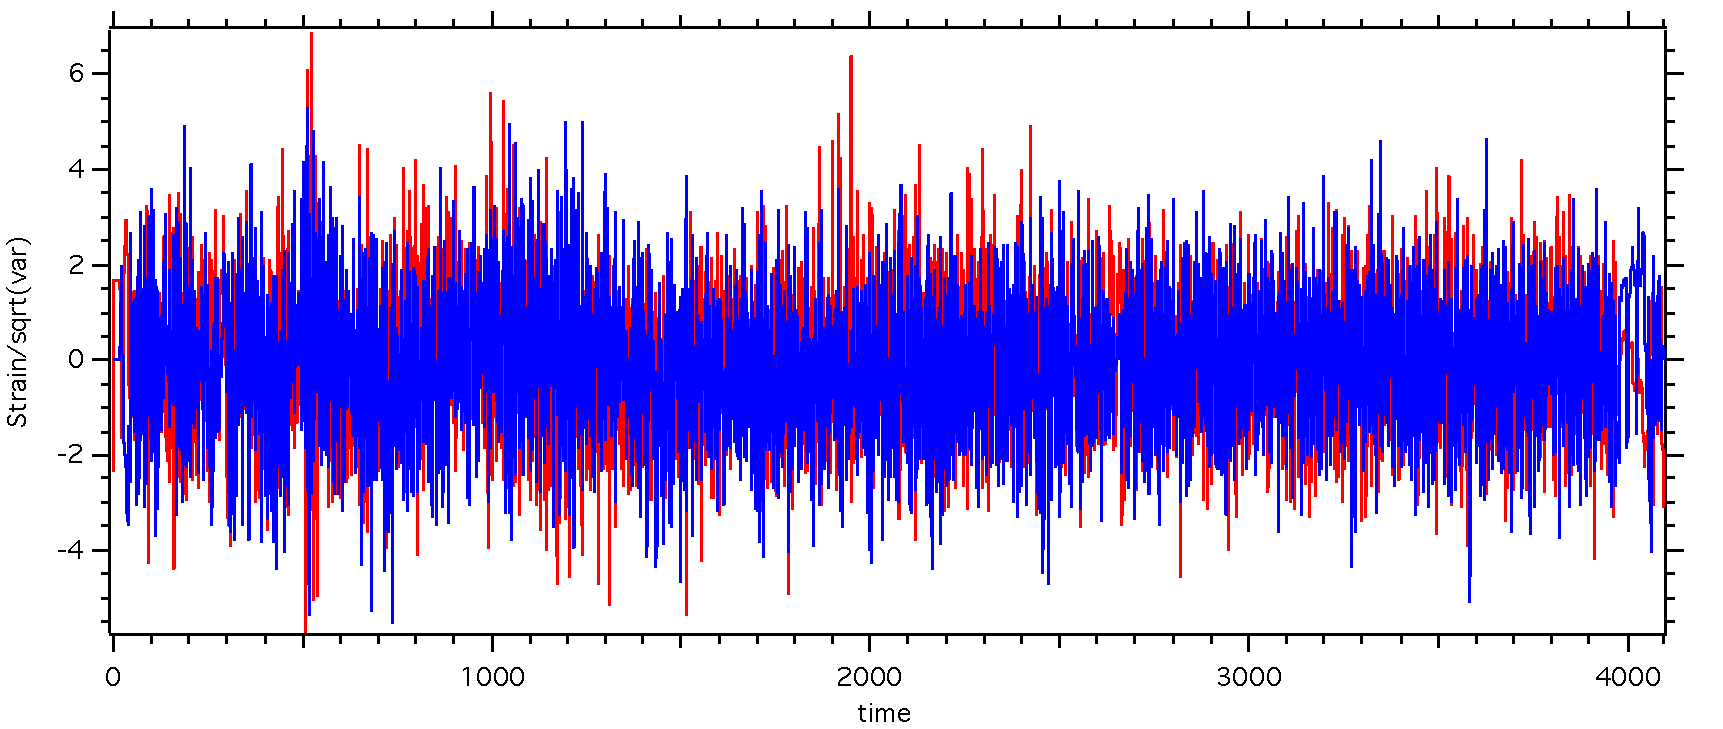
\includegraphics[width=0.8\textwidth]{Figures/strainData.pdf}
   	\caption{Whitened strain data's imaginary (red) and real (blue) parts of the frequency from one observatory. The data is from the first observing run in 2015, and is supposed to contain a candidate event.}
   	\label{Fig:strainData}
   \end{figure}
   
 
 In Figure~\ref{Fig:strainData} we have some data that is considered to contain a candidate event. The figure contains the whitened strain data (the strain data divided by the noise's standard deviation) plotted against the frequency. We obtain the real and the imaginary parts of the frequency by calculating a Fast Fourier Transform of the initial time data as discussed in the previous section.\\
 
 Since the data in Figure~\ref{Fig:strainData} contains a candidate event, the data can be fit by either of the two models:  \mynobreakpar
 \begin{itemize}
 	\item $\mathcal{H}_{GW}$ model - a gravitational wave strain and noise \mynobreakpar
 	\item $\mathcal{H}_{null}$ model - noise that triggered the program to consider it a candidate event
 \end{itemize}
 
 To select which model fits the data better, we can calculate the marginal likelihoods for both the models, with Eq~\ref{eq:evidence}. Since we have data from two observatories, and since in this case, we only look at two parameters, the equation for calculating the marginal likelihood can be re-written for the $\mathcal{H}_{GW}$ model as 
 \begin{align*}
 	P(d_L,d_H | h\propto m_1, m_2) = & \int_{m_1, m_2} { P(m_1,m_2) \ P(m_1,m_2 | d_H)\ dm_1\ dm_2 } \\
 	& \times \int_{m_1, m_2} { P(m_1,m_2) \ P(m_1,m_2 | d_L)\ dm_1\ dm_2 } \ .
 \end{align*}
 
 
 In this equation, the likelihood for the masses $m_1 \text{ and } m_2$ given the data at Hanford and Livingston ($d_H, d_L$) is calculated for each set of values for $m_1,m_2$ ($\forall m_2 < m_1$). After the likelihood is calculated for all sets of masses ($\forall m_2 < m_1$), the evidence is calculated with Eq~\ref{eq:evidence}.\\
 
 
 With the evidence for both models, we calculate the log of the Bayes factor, by modifying Eq~\ref{eq:BayesFactorOrig} to 
 \begin{align*}
\text{log }B_{GW,null} &= \text{log Evidence}_{GW} - \text{log Evidence}_{null} \\
&= 50,000,000.
 \end{align*}
 
  This value suggests to us that there is a higher probability that the data contains a gravitational wave strain and some noise than just noise.\\ 
 
 
    \begin{figure}[h]
    	\centering
    	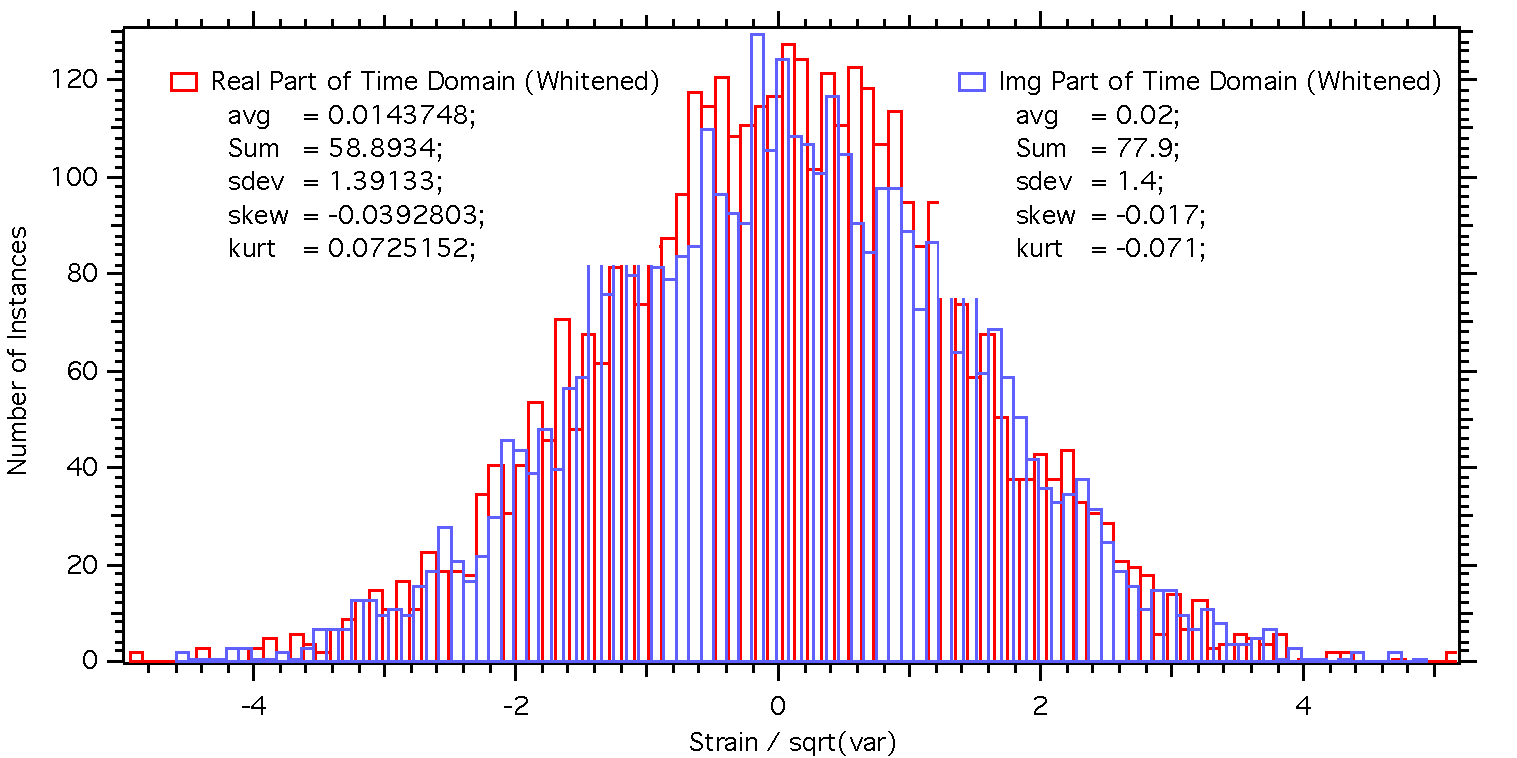
\includegraphics[width=1\textwidth]{Figures/NoiseHistogram.pdf} 
    	\caption{A histogram of strain data that does not have any strain due to a gravitational wave. This shows us that the noise in the data is Gaussian with a zero mean.}
    	\label{Fig:NoiseHist}
    \end{figure}
    
 
 Note that the noise in this data is considered to be a Gaussian with a zero mean, as discussed in section~\ref{section:introToBayes}. This is because if we plot strain data that contains only noise, and create a histogram of the data, we get a plot as seen in Figure~\ref{Fig:NoiseHist}. This is a Gaussian with a mean of $\mu \approx 0$. In most cases, the data that is recorded is mostly noise, and even data with gravitational wave strains appear to look like they only have noise. It is with the various analysis methods that we can find out is the data contains anything other than noise.\\
  
 
 
 \subsubsection{Parameter Estimation}
 
     \begin{figure}[h]
     	\centering
     	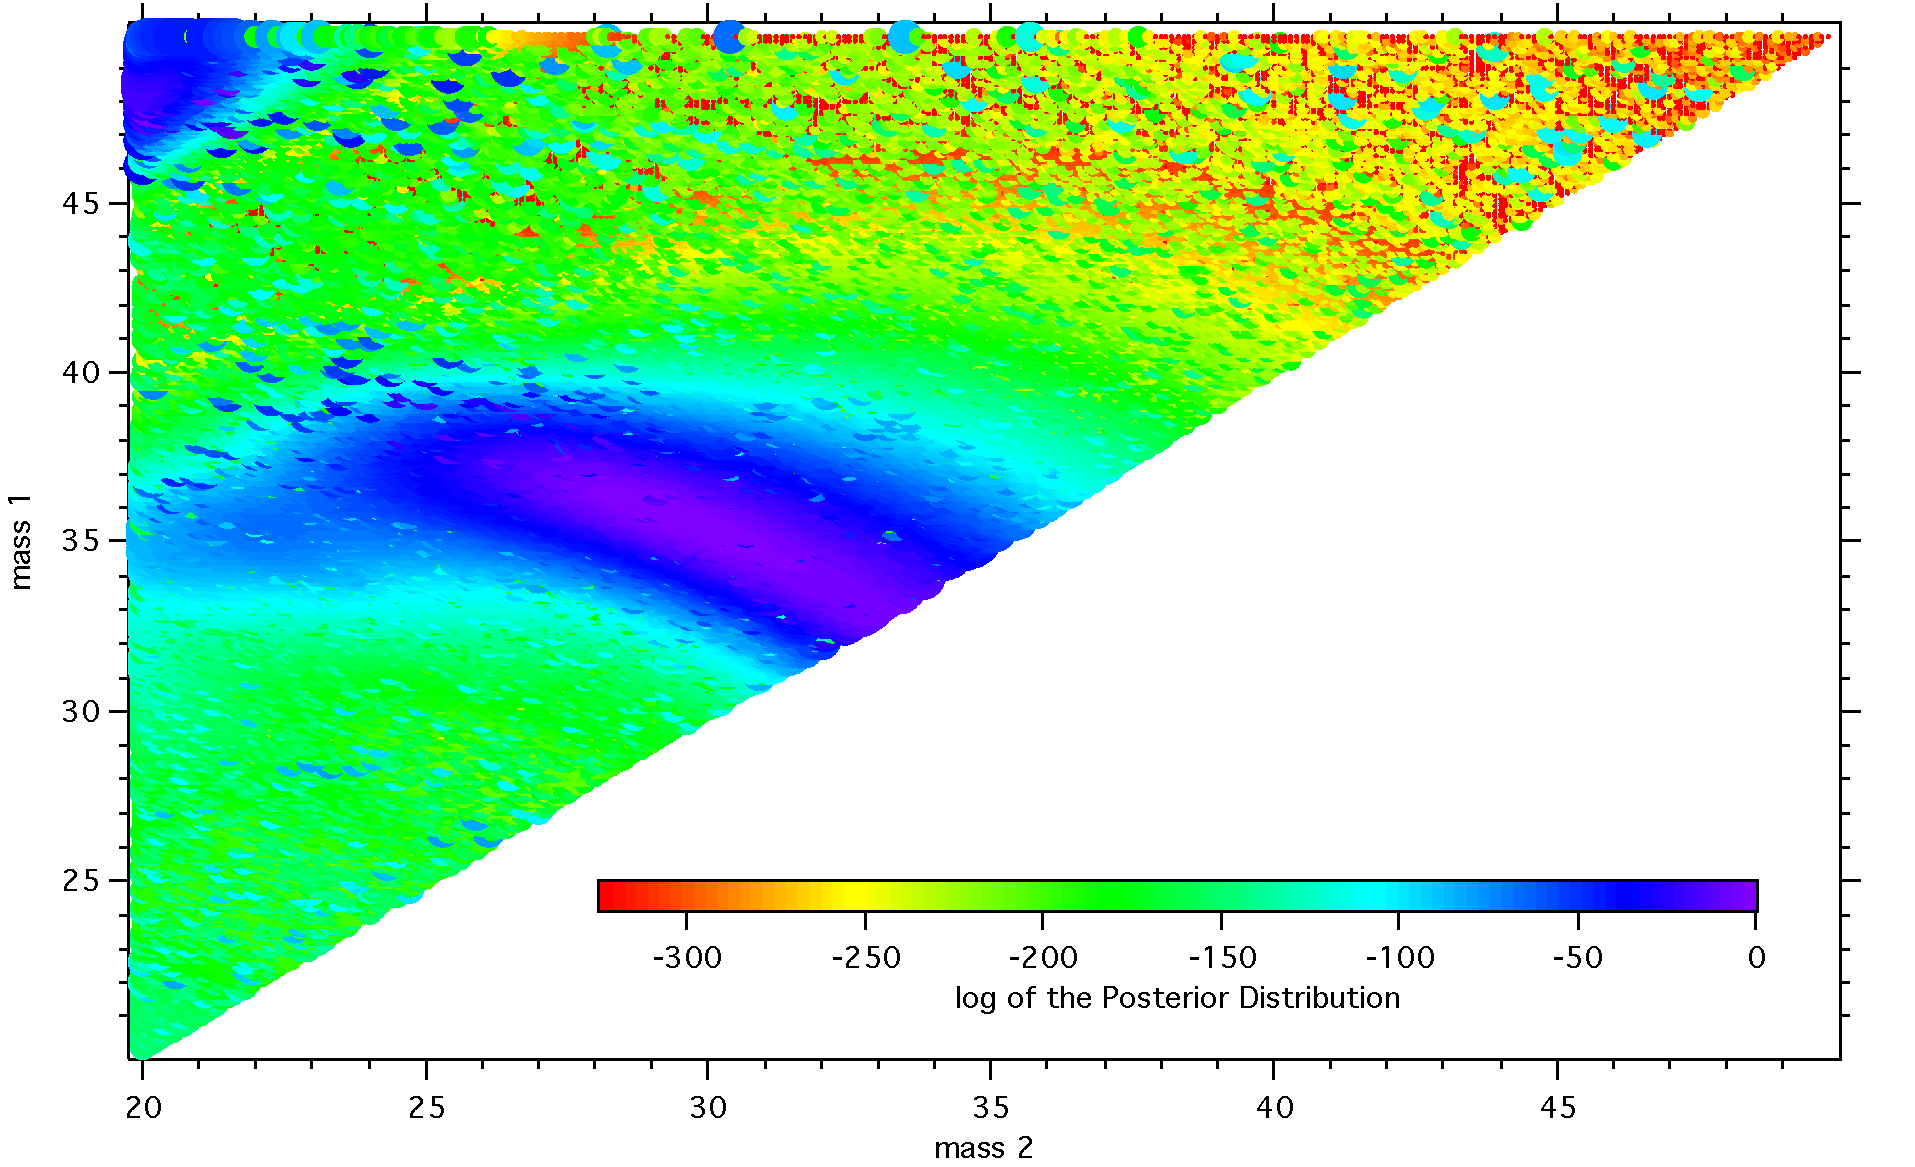
\includegraphics[width=1\textwidth]{Figures/m1m2.pdf} 
     	\caption{2D plot of the log of the posterior distribution for the masses of the black holes before the merger. We can see a high posterior region near the 30-38 solar mass range. The data for this was generated from an injected gravitational wave strain.}
     	\label{Fig:2Dmasses}
     \end{figure}
 
 Now that we know that the candidate event actually contains a signal, we can use the data for the posteriors we calculated when we were calculating the Marginal likelihood to calculate the posterior distribution for parameters. Here we calculate the posterior distributions for the masses of the merging binary black holes. Using Eq~\ref{eq:PDF} and \ref{eq:likelihood}, if we plot the likelihoods for the entire set of combinations of the masses, we can get a plot as seen in Figure~\ref{Fig:2Dmasses}. This tells us that the masses of the black holes are most likely to be in the range of 30 - 37 solar masses in size. Note that the plot does not include the posterior density for all the combination of masses. This is because after the diagonal, the combinations of the masses would be repeated. \\
 
     \begin{figure}[h]
     	\centering
     	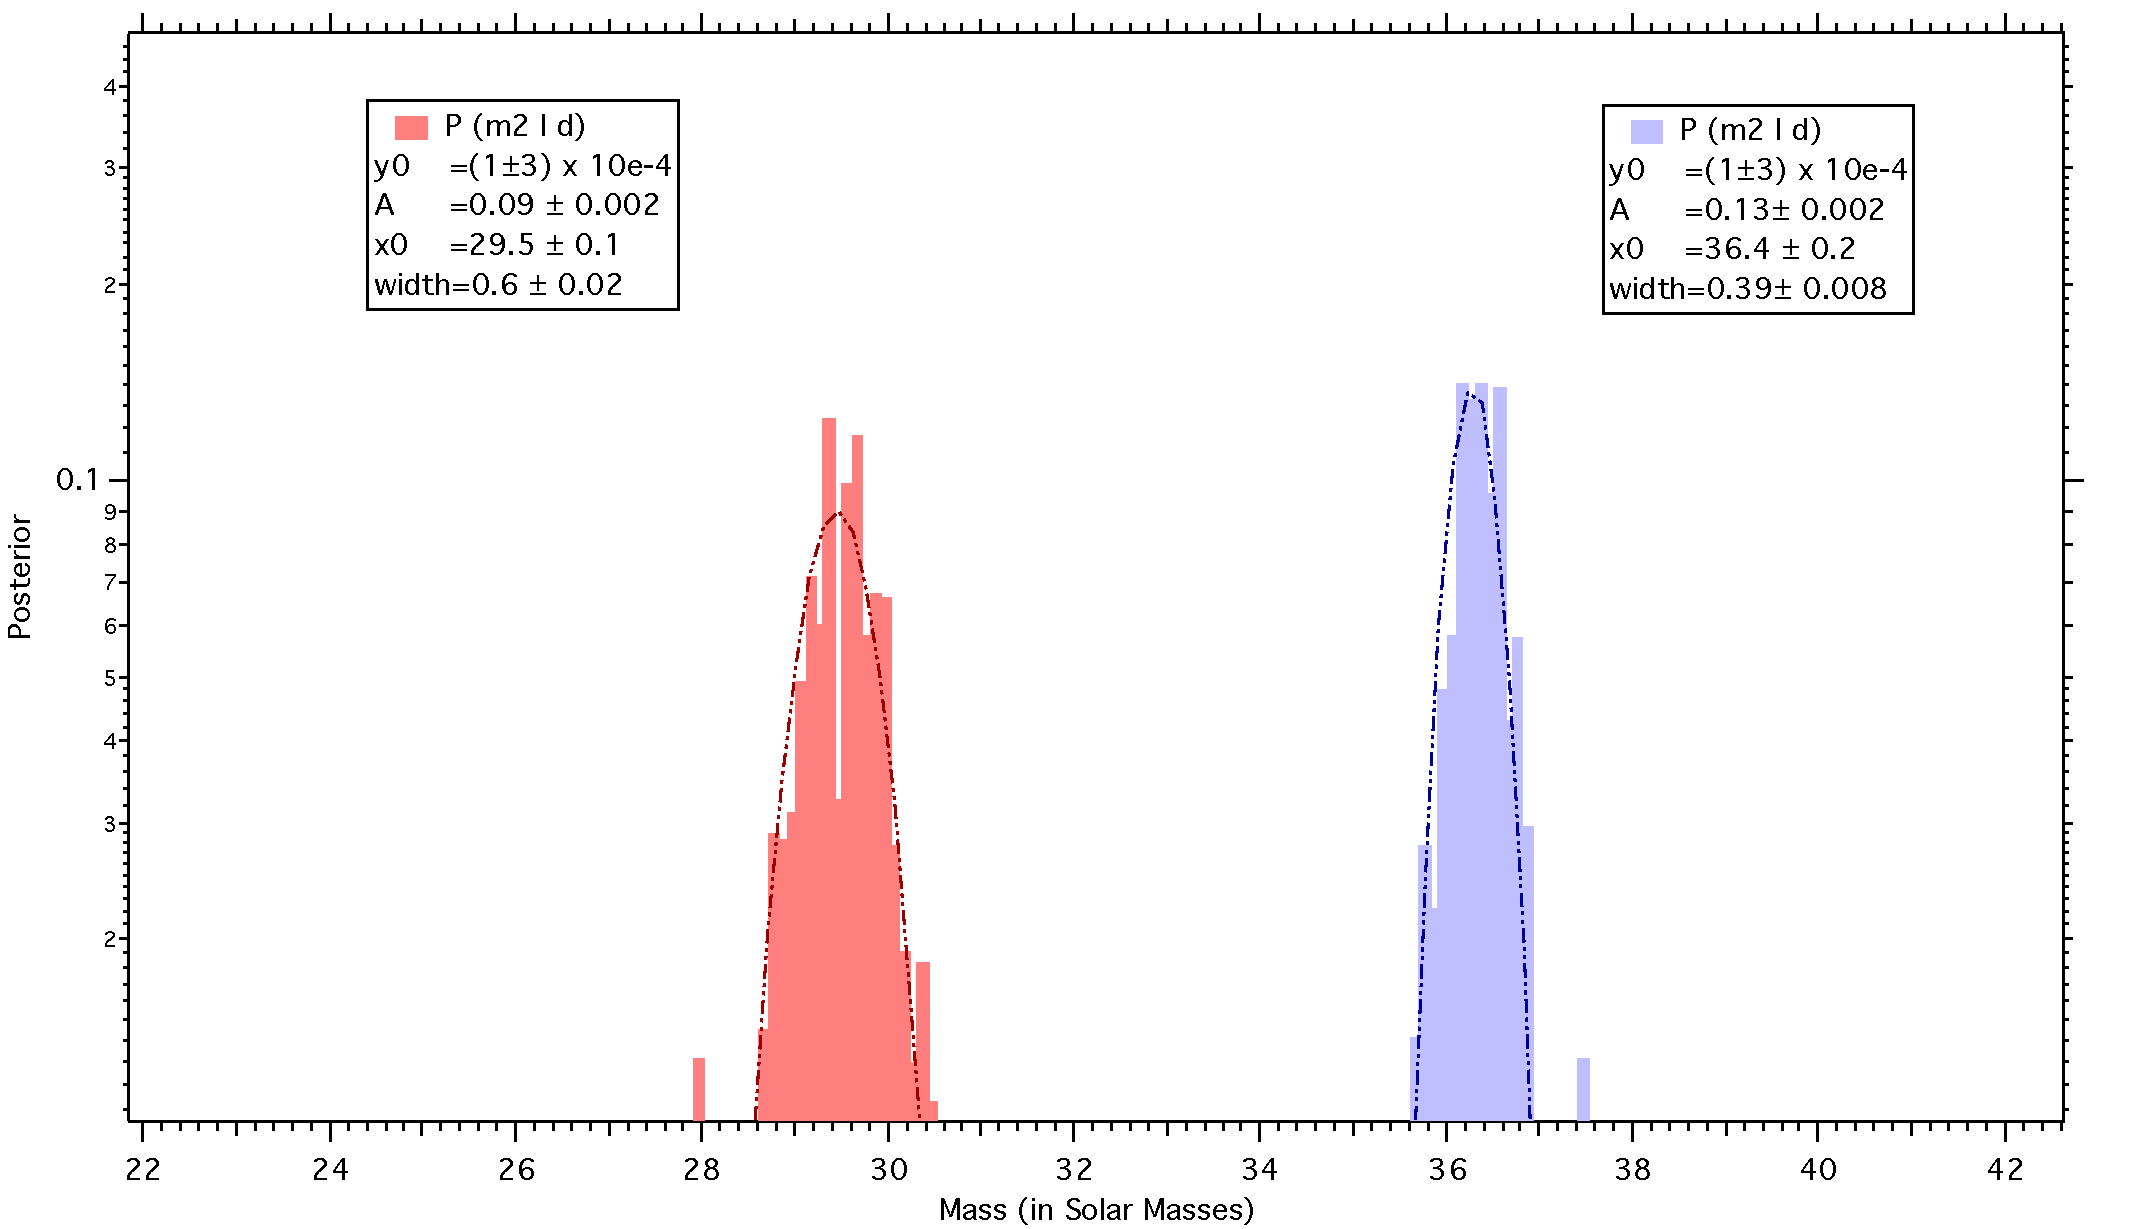
\includegraphics[width=1\textwidth]{Figures/MassPost.pdf} 
     	\caption{Posteriors for the masses of the black holes before the  merger. This was created with data from an injected gravitational wave strain. The masses  of the black holes are $29.5\pm0.1 \text{ and } 36.4\pm0.2$ solar masses in size.}
     	\label{Fig:1Dmasses}
     \end{figure}
 
 
 To get a better estimation on what the mass for each black hole may be, we can integrate out the posterior for both masses, with the equation $$P(m_1|d)= \int_{m_2} {P(m_1, m_2 | d) dm_2}.$$ The plot of the posterior density of the masses can be studied in Figure~\ref{Fig:1Dmasses}. From this, we can conclude that the masses for the black holes are approximately $29.5\pm0.1 \text{ and } 36.4\pm0.2$ solar masses in size. This method is similar to how parameter estimation is done for all the parameters for a gravitational wave signal. A discussion on how a gravitational wave signal is analysed for all the parameters is done in the next section.\\
 
 
 \subsection{Running LALinference to Analyse A Candidate Event}
 
 To analyse a candidate event, such as the one seen in Fig~\ref{Fig:DataLH}, there have been scripts written that use several computers to compare numerous waveform templates with the signal data. The templates are different for each parameter set, and once a certain number of templates are run for various parameters, numerous plots of posterior destinies for various parameters along with other information regarding the candidate event are displayed on a results page. \\
 
 
 
 \begin{figure}[h]
 	\centering
 	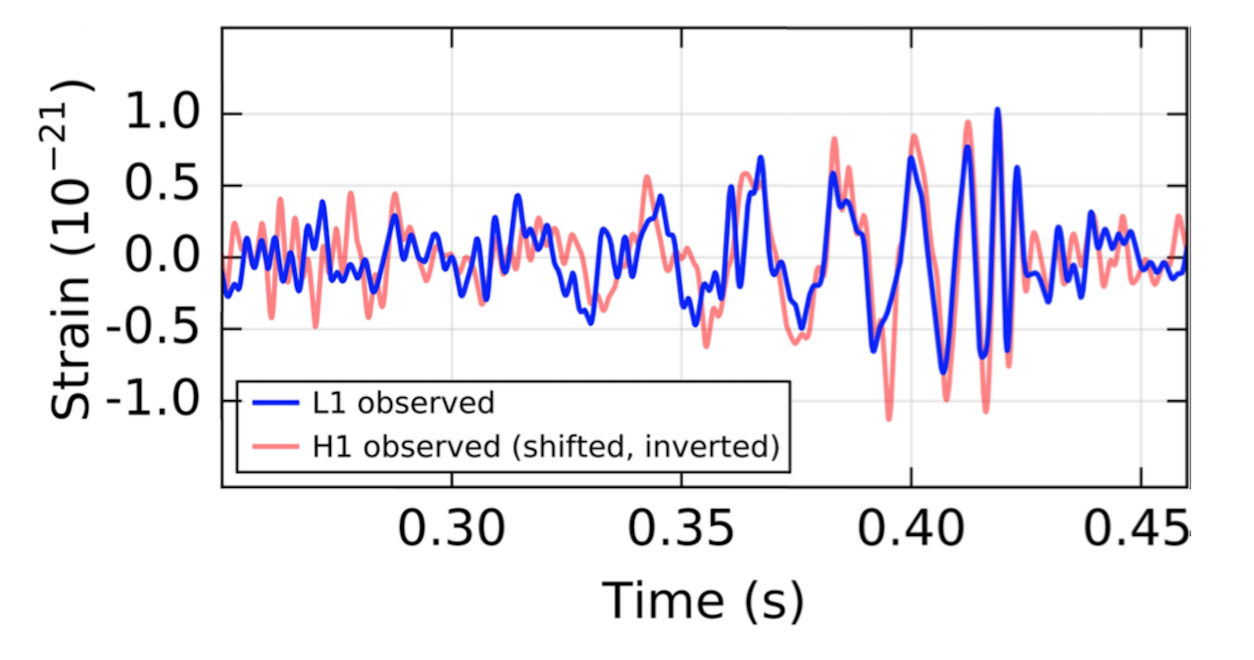
\includegraphics[width=0.7\textwidth]{Figures/DataLH.png} 
 	\caption{The filtered instrumental strain data in the Livingston detector (blue) and Hanford detector (red). The Hanford strain has been shifted back in time by 6.9 ms and inverted. This figure was taken from Ref~\cite{ligo2016properties}.
 	}
 	\label{Fig:DataLH}
 \end{figure}
 
 
 Depending on the initial parameters passed to the function to analyse the candidate event, the results page will include the log of the Bayes factor and the Bayes factor of the gravitational wave strain model against the noise model. This value helps us decided if the candidate event has information regarding a gravitational wave strain, or if it contains just noise. \\
 
 
 This sections discusses an analysis of the $GW150914$ gravitational wave, detected during the first observatory run of aLIGO. This analysis was conducted with the `lalinference$\_$nest' script, which uses a Nested Sampling algorithm to calculate the evidence. \\
 
 The nested sampling algorithm randomly pick sets of parameters in $\vec{\theta}$, and first calculates likelihoods for each set of parameters. Once a certain amount of likelihoods are calculated, the algorithm calculates the evidence using the several sets of likelihoods. If the value of the evidence is below a certain threshold set before running the script, the nested sampling algorithm chooses another set of values of the parameters in $\vec{\theta}$ and calculates the likelihood and the evidence again with the new set of parameters, along with the rest of the old sets of parameters. Note that after the initial sets of parameters are chosen, the new set of parameters are used for the calculations only if the likelihood for the new parameter set is a value above a certain amount. This process of picking a set of the new parameter sets is repeated until the likelihoods are the maximum ones present in the parameter space.\\
 
 
  On running the analysis, we received a Bayes Factor of $5.77\times 10^{36}$, which suggests that there is a some gravitational wave strain signal present in the data.\\
 
      \begin{figure}[h]
      	\centering
      	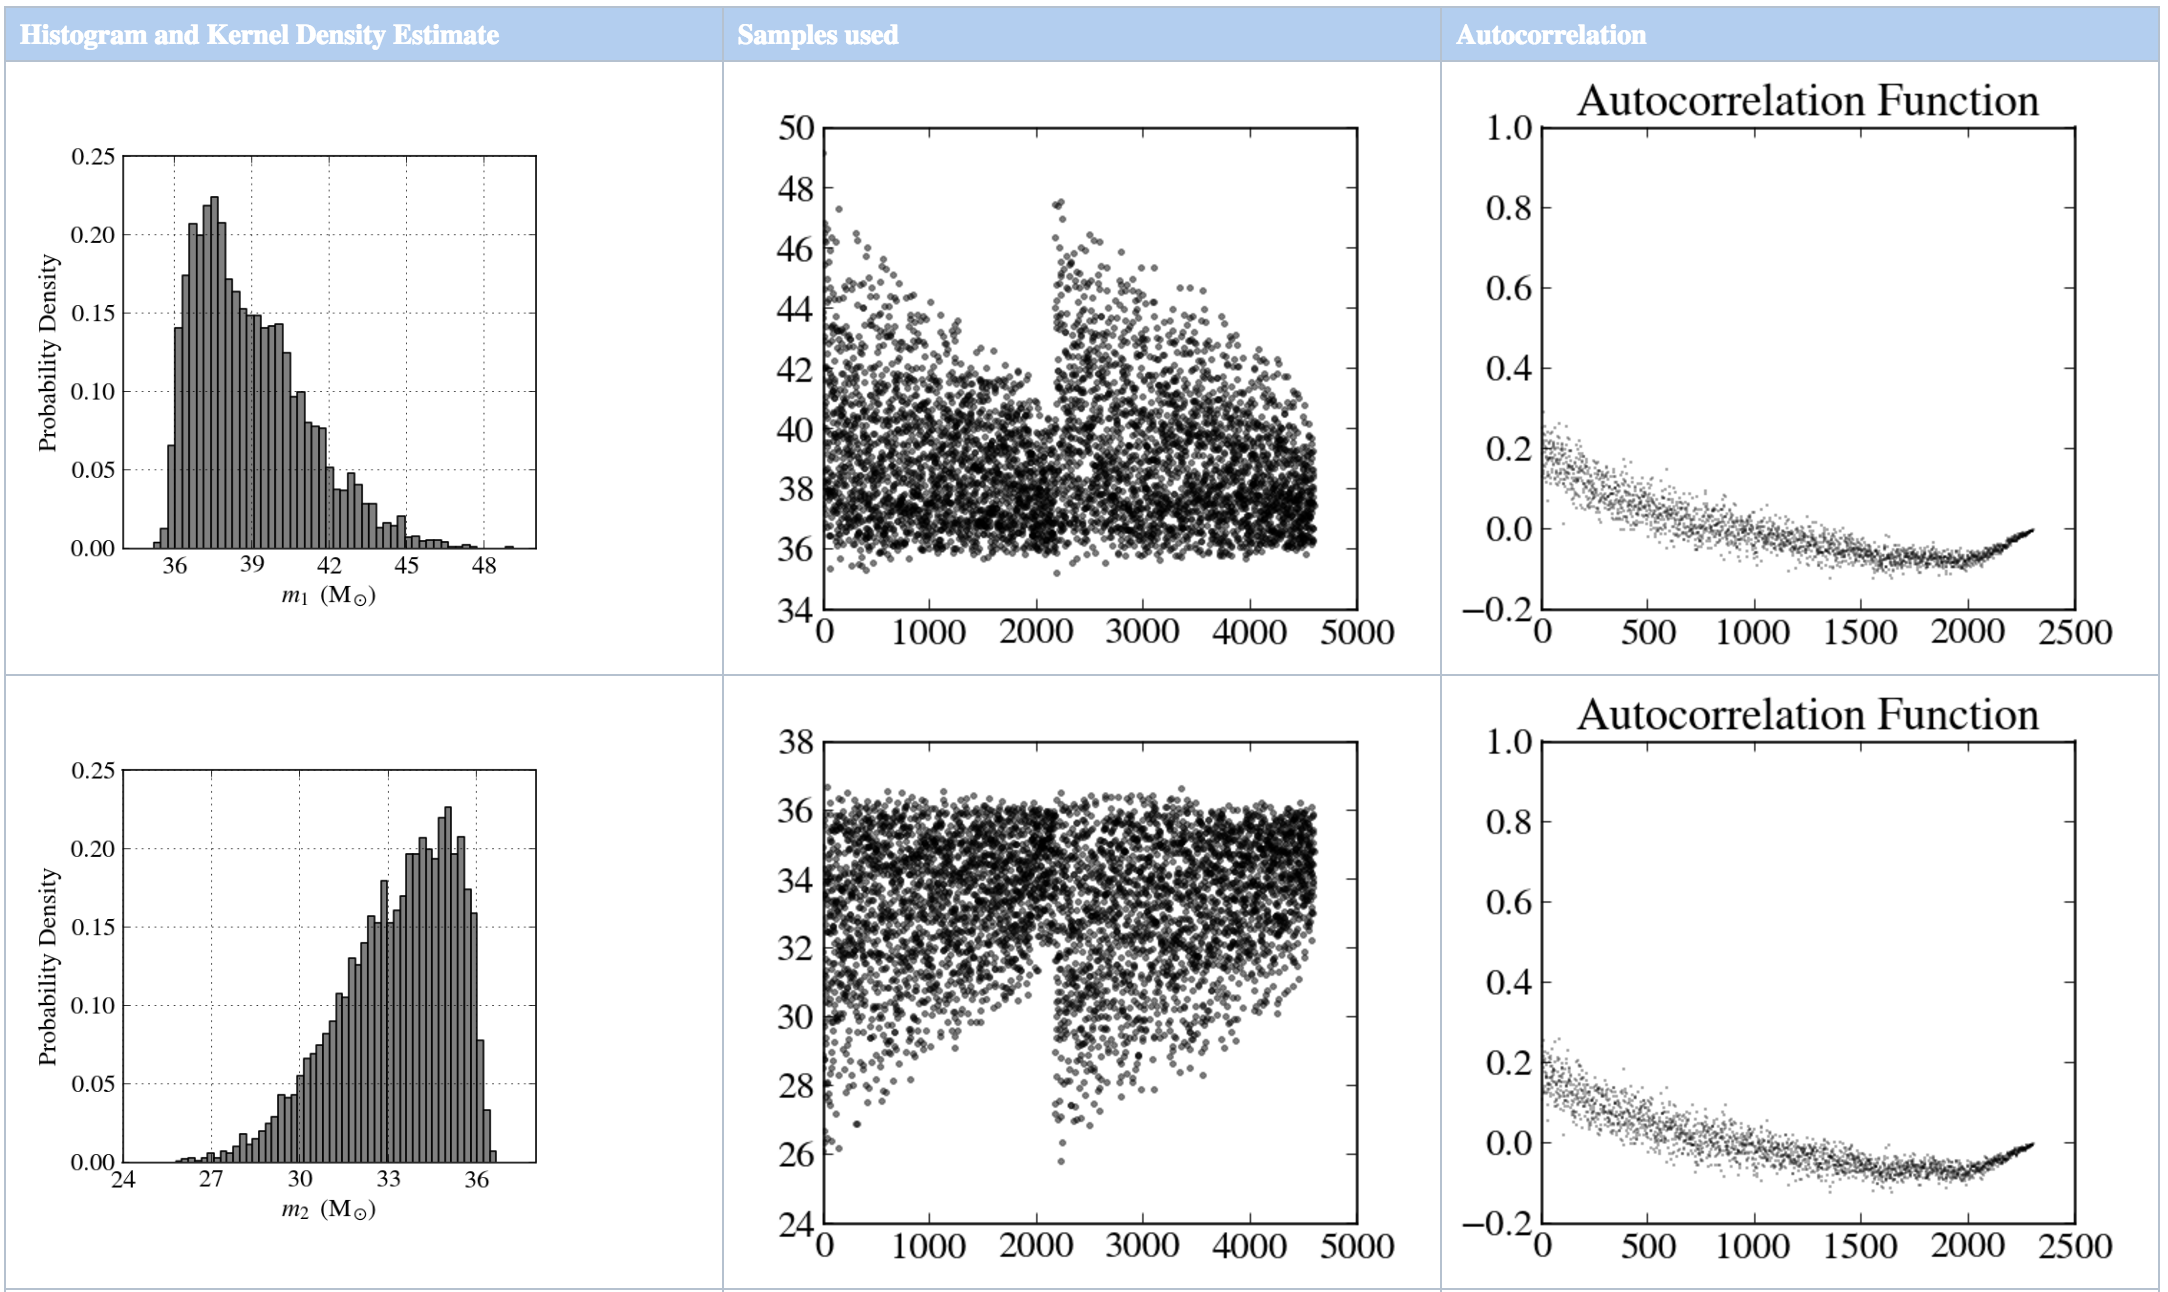
\includegraphics[width=1\textwidth]{Figures/LALinferenceMasses.png} 
      	\caption{Posteriors for the black hole masses before the merger, created with the LALinference script. The masses are $39.5\pm3.2 \text{ and } 32.4\pm2.7$ solar masses in size. The data used for this was the same as the data from the $GW150914$ detection.}
      	\label{Fig:LALinferenceMasses}
      \end{figure}
      
      
 As the data contains a gravitational wave, we were able to calculate various parameters such as the masses, spins and orientations of the black holes. Figure~\ref{Fig:LALinferenceMasses} contains plots of the masses of the black holes, which tell us that the masses of the black holes were $39.5\pm3.2 \text{ and } 32.4\pm2.7$ solar masses. Several plots similar to the one in Figure~\ref{Fig:LALinferenceMasses} were generated for the other parameters of the binary black hole system. These help us state what values we believe that the system has. 
 
 We will run this analysis for several sets of instances where no gravitational wave strain is present to calculate the Bayes factor for these instances. As no gravitational waves are present in this data, we can create a background distribution of the value that we expect the Bayes factor to be if no gravitational wave data is present in the strain data. We will then run this analysis for the several candidate events that we observed to see if they have higher Bayes factors than the background distribution. 
 
% \section{Other things to write about}
% 
% \begin{itemize}
% 	\item nested sampling 
% 	\item a basis vector to calculate the hOfF faster
% 	\item  Lit review and the VV paper, Text, Param estimation paper, Basics physics of Binary Black Hole Mergers Paper.
% 	\item  talk about False alarma events, corellated and realated
% \end{itemize}
 

 
 
% % Figure for example m
% \begin{figure}[h]
% 	\centering
% 	
% 
 % Figure for Example G search 
 %- Strain
 % Whitened Data
 % Mass vs mass
 % mass prob
 
 
 %----------------------------------------------------------------------------------------
 %	SECTION 4
 %----------------------------------------------------------------------------------------
 
 
 \section{Project Schedule}
 
 
 \textbf{WEEK 1:} Restructure the problem statement, and understand the past programming done for Bayesian statistics. Develop an approach to write the program to create the detection statistic that will rank the events using the Bayes factor defined in Eq~\ref{eq:BayesFactorOrig}.\\
 \textbf{WEEK 2-3:} Analyse noise and injected gravitational wave signals to determine sensitivity of the Bayes Factor.\\
 \textbf{WEEK 4:} Study the results in detail, and restructure the computer program. Test the thresholds and compare the Bayes Factor detection statistic to the SNR detection statistic. \\
  \textbf{WEEK 6-7:} Understand the results and collect more data. Begin compiling figures and writing to make the work more presentable. \\
  \textbf{WEEK 8-9:} Further documentation of the lab notebook, and program, for future researchers. Begin retaking data if required for the final paper.\\
 
 
 
 
 %----------------------------------------------------------------------------------------
 %	REFERENCES
 %----------------------------------------------------------------------------------------
 
---------------------------------------------------------------------
 
 \bibliographystyle{plain}		% Using this bibliography style will ignore the annotations.
 
 \bibliography{ProjectProposalRefrences}
 
%----------------------------------------------------------------------------------------


\end{document}